\documentclass[letterpaper, 12pt]{texMemo}
\usepackage[american]{babel}
\usepackage{graphicx}
\usepackage[citestyle=apa,style=apa,backend=biber]{biblatex}
\DeclareLanguageMapping{american}{american-apa}
\addbibresource{bibliography.bib}
\memoto{Dr. William Hsu}
\memofrom{Blair Urish}
\memosubject{Visual Aids}
\memodate{February 27, 2017}

\begin{document}
\maketitle
\begin{flushleft}
\subsection*{Introduction}
The purpose of this memo is to provide examples of two visual aids that will be used in this literature review. Justifications for the inclusion of the visual aids is also given.

\subsection*{Figure 1}
This figure identifies the 3 layers of the Internet of Things architecture. It provides the reader with examples of services that function at each layer.


\begin{figure}[h!]
	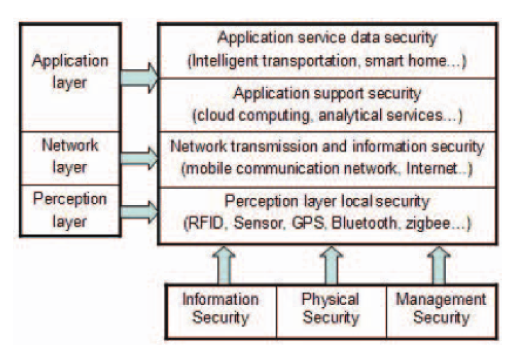
\includegraphics[width=\linewidth]{figure2.png}
	\caption{Internet of Things Architecture}
	\label{fig:arch}
\end{figure}

\subsection*{Justification for Figure 1}
It is important for the reader to understand the differences between each of the layers of the Internet of Things Architecture. 
This figure provides examples of devices commonly found in each layer and what type of security is necessary. 

\newpage
Bibliography\\
~\newline
  \fullcite{Zhao6746513}
\end{flushleft}
\end{document}
